% ═══════════════════════════════════════════════════════════════════════════════
\section{Konformitätsstufen}
\label{sec:konformitaet}
% ═══════════════════════════════════════════════════════════════════════════════

Der UQTL-Standard definiert vier Konformitätsstufen (Conformance Levels),
die eine schrittweise Implementierung ermöglichen. Höhere Stufen schließen
alle Anforderungen niedrigerer Stufen ein.

\begin{figure}[H]
\centering
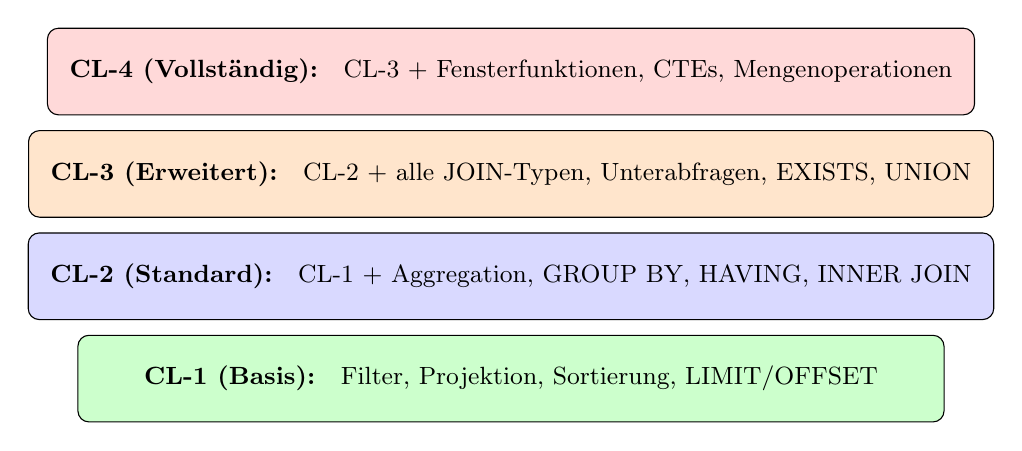
\begin{tikzpicture}[
  level/.style={draw, rounded corners=4pt, minimum width=11cm,
    minimum height=1.1cm, align=left, font=\small,
    inner sep=8pt},
  cl1/.style={level, fill=green!20},
  cl2/.style={level, fill=blue!15},
  cl3/.style={level, fill=orange!20},
  cl4/.style={level, fill=red!15},
]
  \node[cl1] (l1) at (0,0)   {\textbf{CL-1 (Basis):}~~~Filter, Projektion, Sortierung, LIMIT/OFFSET};
  \node[cl2] (l2) at (0,1.3) {\textbf{CL-2 (Standard):}~~~CL-1 + Aggregation, GROUP BY, HAVING, INNER JOIN};
  \node[cl3] (l3) at (0,2.6) {\textbf{CL-3 (Erweitert):}~~~CL-2 + alle JOIN-Typen, Unterabfragen, EXISTS, UNION};
  \node[cl4] (l4) at (0,3.9) {\textbf{CL-4 (Vollständig):}~~~CL-3 + Fensterfunktionen, CTEs, Mengenoperationen};
\end{tikzpicture}
\caption{UQTL-Konformitätspyramide (CL-1 bis CL-4)}
\label{fig:konformitaet}
\end{figure}

\subsection{CL-1: Basiskonformität}
\label{subsec:cl1}

Ein CL-1-konformes System muss die folgenden Operatoren vollständig und
äquivalenzerhaltend unterstützen:

\begin{itemize}[leftmargin=1.5cm]
  \item \textbf{SCAN:} Zugriff auf einzelne Tabellen mit optionalem Alias
  \item \textbf{FILTER (WHERE):} Alle Vergleichsoperatoren ($=$, $\neq$, $<$, $\leq$, $>$, $\geq$),
    \texttt{IN}, \texttt{BETWEEN}, \texttt{LIKE}, \texttt{IS NULL}, \texttt{AND}, \texttt{OR}, \texttt{NOT}
  \item \textbf{PROJECT:} Spaltenselektion, Ausdrücke, \texttt{DISTINCT}
  \item \textbf{SORT:} \texttt{ORDER BY} ASC/DESC, mehrstufig
  \item \textbf{LIMIT:} \texttt{LIMIT n OFFSET m}
\end{itemize}

\subsection{CL-2: Standardkonformität}
\label{subsec:cl2}

Zusätzlich zu CL-1 müssen CL-2-konforme Systeme unterstützen:

\begin{itemize}[leftmargin=1.5cm]
  \item \textbf{GROUP\_AGG:} \texttt{GROUP BY}, alle Standardaggregationen (\texttt{COUNT}, \texttt{SUM}, \texttt{AVG}, \texttt{MIN}, \texttt{MAX})
  \item \textbf{FILTER (HAVING):} Aggregatprädikate nach \texttt{GROUP BY}
  \item \textbf{JOIN (INNER):} \texttt{INNER JOIN ... ON}, \texttt{NATURAL JOIN}
  \item \textbf{Arithmetische Ausdrücke} in Projektionen und Prädikaten
\end{itemize}

\subsection{CL-3: Erweiterte Konformität}
\label{subsec:cl3}

Zusätzlich zu CL-2:

\begin{itemize}[leftmargin=1.5cm]
  \item \textbf{JOIN (alle Typen):} \texttt{LEFT/RIGHT/FULL OUTER JOIN}, \texttt{CROSS JOIN}
  \item \textbf{SUBQUERY:} Korrelierte und nicht-korrelierte Unterabfragen, Scalar Subqueries
  \item \textbf{EXISTS / NOT EXISTS}
  \item \textbf{SET\_OP:} \texttt{UNION}, \texttt{UNION ALL}
  \item \textbf{Skalare Funktionen:} Zeichenkettenfunktionen, Datumsfunktionen, mathematische Funktionen
\end{itemize}

\subsection{CL-4: Vollständige Konformität}
\label{subsec:cl4}

Zusätzlich zu CL-3:

\begin{itemize}[leftmargin=1.5cm]
  \item \textbf{WINDOW:} Alle ANSI-Fensterfunktionen (\texttt{ROW\_NUMBER}, \texttt{RANK}, \texttt{DENSE\_RANK}, \texttt{LAG}, \texttt{LEAD}, \texttt{FIRST\_VALUE}, \texttt{LAST\_VALUE}, \texttt{NTH\_VALUE}, gleitende Aggregate)
  \item \textbf{WITH (CTEs):} Einfache und rekursive CTEs
  \item \textbf{SET\_OP vollständig:} \texttt{INTERSECT}, \texttt{EXCEPT}
  \item \textbf{CASE-Ausdrücke}
  \item \textbf{Dialekt-Erweiterungen} (als optionale Zertifizierung)
\end{itemize}

\begin{table}[H]
\centering
\caption{Konformitätsstufen-Übersicht}
\label{tab:konformitaet}
\renewcommand{\arraystretch}{1.3}
\begin{tabularx}{\textwidth}{lXXXX}
\toprule
\textbf{Feature} & \textbf{CL-1} & \textbf{CL-2} & \textbf{CL-3} & \textbf{CL-4} \\
\midrule
Filter (WHERE) & \checkmark & \checkmark & \checkmark & \checkmark \\
Projektion & \checkmark & \checkmark & \checkmark & \checkmark \\
Sortierung & \checkmark & \checkmark & \checkmark & \checkmark \\
LIMIT/OFFSET & \checkmark & \checkmark & \checkmark & \checkmark \\
GROUP BY / Aggregation & & \checkmark & \checkmark & \checkmark \\
HAVING & & \checkmark & \checkmark & \checkmark \\
INNER JOIN & & \checkmark & \checkmark & \checkmark \\
OUTER JOINs & & & \checkmark & \checkmark \\
Unterabfragen & & & \checkmark & \checkmark \\
EXISTS & & & \checkmark & \checkmark \\
UNION / UNION ALL & & & \checkmark & \checkmark \\
Fensterfunktionen & & & & \checkmark \\
CTEs (WITH) & & & & \checkmark \\
INTERSECT / EXCEPT & & & & \checkmark \\
CASE-Ausdrücke & & & & \checkmark \\
\bottomrule
\end{tabularx}
\end{table}

% ═══════════════════════════════════════════════════════════════════════════════
\section{Referenzimplementierung}
\label{sec:implementierung}
% ═══════════════════════════════════════════════════════════════════════════════

\subsection{Architektur einer UQTL-konformen Implementierung}
\label{subsec:impl_arch}

Eine UQTL-konforme Implementierung besteht aus drei Schichten:

\begin{enumerate}[leftmargin=1.5cm]
  \item \textbf{Frontend-Parser:} Sprach\-spezifische Analyse und
    IQT-Aufbau (je ein Parser pro Quellsprache)
  \item \textbf{IQT-Normalisierer:} Anwendung der Normalisierungsregeln
    (\ref{subsec:iqt_norm})
  \item \textbf{SQL-Codegenerator:} IQT-zu-SQL-Übersetzung nach Zieldialekt
\end{enumerate}

\subsection{Pseudocode des IQT-Builders (Python-Frontend)}
\label{subsec:impl_py}

\begin{lstlisting}[style=pythonstyle, caption={Python-Frontend: IQT-Builder (vereinfacht)},
  label=lst:impl_py]
class PythonIQTBuilder:
    """Baut einen IQT-Baum aus einem SQLAlchemy Select-Statement."""

    def build(self, stmt: Select) -> IQTNode:
        node = self._visit_froms(stmt)          # SCAN / JOIN
        node = self._visit_where(stmt, node)    # FILTER WHERE
        node = self._visit_group_having(stmt, node)  # GROUP_AGG + HAVING
        node = self._visit_select(stmt, node)   # PROJECT
        node = self._visit_order(stmt, node)    # SORT
        node = self._visit_limit(stmt, node)    # LIMIT
        return node

    def _visit_where(self, stmt, source):
        if stmt.whereclause is not None:
            pred = self._translate_predicate(stmt.whereclause)
            return FilterNode(source=source, predicate=pred,
                              position=FilterPosition.WHERE)
        return source

    def _translate_predicate(self, clause) -> IQTExpr:
        if isinstance(clause, BinaryExpression):
            left  = self._translate_expr(clause.left)
            right = self._translate_expr(clause.right)
            op    = self._map_operator(clause.operator)
            return CompareExpr(left=left, op=op, right=right)
        elif isinstance(clause, BooleanClauseList):
            children = [self._translate_predicate(c) for c in clause.clauses]
            logic = LogicOp.AND if clause.operator == operators.and_ \
                    else LogicOp.OR
            return LogicExpr(op=logic, operands=children)
        # ... weitere Faelle
\end{lstlisting}

\subsection{Pseudocode des SQL-Codegenerators}
\label{subsec:impl_codegen}

\begin{lstlisting}[style=pythonstyle, caption={SQL-Codegenerator: IQT nach ANSI SQL},
  label=lst:impl_codegen]
class AnsiSqlCodegen:
    """Generiert ANSI SQL:2016 aus einem normalisierten IQT."""

    def generate(self, node: IQTNode) -> str:
        parts = self._collect(node)
        return self._assemble(parts)

    def _collect(self, node, parts=None) -> SqlParts:
        if parts is None:
            parts = SqlParts()

        if isinstance(node, ScanNode):
            parts.from_clause = f"{node.table} AS {node.alias}"

        elif isinstance(node, FilterNode):
            self._collect(node.source, parts)
            pred_sql = self._gen_expr(node.predicate)
            if node.position == FilterPosition.WHERE:
                parts.where_clauses.append(pred_sql)
            else:
                parts.having_clauses.append(pred_sql)

        elif isinstance(node, JoinNode):
            self._collect(node.left, parts)
            right_sql  = f"{node.right.table} AS {node.right.alias}"
            cond_sql   = self._gen_expr(node.condition.predicate)
            join_kw    = JOIN_KEYWORDS[node.join_type]
            parts.joins.append(f"{join_kw} {right_sql} ON {cond_sql}")

        elif isinstance(node, GroupAggNode):
            self._collect(node.source, parts)
            parts.group_by = ", ".join(
                self._gen_expr(e) for e in node.group_by)
            parts.select_items.extend(
                f"{self._gen_agg(a)} AS {a.alias}" for a in node.aggregates)

        elif isinstance(node, ProjectNode):
            self._collect(node.source, parts)
            parts.distinct = node.distinct
            parts.select_items = [
                self._gen_proj(item) for item in node.columns]

        elif isinstance(node, SortNode):
            self._collect(node.source, parts)
            parts.order_by = ", ".join(
                self._gen_sort_item(s) for s in node.items)

        elif isinstance(node, LimitNode):
            self._collect(node.source, parts)
            if node.count is not None:
                parts.limit  = str(self._gen_expr(node.count))
            if node.offset is not None:
                parts.offset = str(self._gen_expr(node.offset))

        return parts

    def _assemble(self, p: SqlParts) -> str:
        distinct = "DISTINCT " if p.distinct else ""
        sel = ", ".join(p.select_items) if p.select_items else "*"
        sql = f"SELECT {distinct}{sel}\nFROM {p.from_clause}"
        if p.joins:
            sql += "\n" + "\n".join(p.joins)
        if p.where_clauses:
            sql += "\nWHERE " + "\n  AND ".join(p.where_clauses)
        if p.group_by:
            sql += f"\nGROUP BY {p.group_by}"
        if p.having_clauses:
            sql += "\nHAVING " + "\n  AND ".join(p.having_clauses)
        if p.order_by:
            sql += f"\nORDER BY {p.order_by}"
        if p.limit:
            sql += f"\nLIMIT {p.limit}"
        if p.offset:
            sql += f"\nOFFSET {p.offset}"
        return sql
\end{lstlisting}

\subsection{Konformitätstests}
\label{subsec:impl_tests}

Eine UQTL-Referenzimplementierung muss eine Test-Suite bestehen, die für
jede Konformitätsstufe die semantische Äquivalenz der Übersetzungen prüft:

\begin{lstlisting}[style=pythonstyle, caption={Konformitätstest-Schablone},
  label=lst:impl_test]
class UQTLConformanceTest:

    def assert_equivalent(self, py_stmt, java_iqt, cs_iqt, expected_sql):
        """Prueft semantische Aequivalenz aller drei Uebersetzungen."""
        py_sql   = PythonIQTBuilder().build(py_stmt)
                   |> IQTNormalizer().normalize()
                   |> AnsiSqlCodegen().generate()
        java_sql = java_iqt
                   |> IQTNormalizer().normalize()
                   |> AnsiSqlCodegen().generate()
        cs_sql   = cs_iqt
                   |> IQTNormalizer().normalize()
                   |> AnsiSqlCodegen().generate()

        assert py_sql   == expected_sql, f"Python divergiert:\n{py_sql}"
        assert java_sql == expected_sql, f"Java divergiert:\n{java_sql}"
        assert cs_sql   == expected_sql, f"C# divergiert:\n{cs_sql}"
\end{lstlisting}
